\section{Auswertung}

Die Größenmessung der Gegenstads- und der Bildgröße wurde mit einem Geodreieck durchgeführt.
Die weiteren Messwerte wurden an einem Lineal, welches an der Schiene integriert
ist, abgelesen. Es wird ein Ablesefehler von $\SI{0,05}{\centi\meter}$ angenommen.
Anhand der genommenen Messwerte wird die Linsengleichung \eqref{eqn:} und das
Abbildungsgesetz \eqref{eqn:} überprüft.

Damit das Abbildungsgesetz überprüft werden kann, sind die Mittelwerte der Messung
der Gegenstands- und der Bildweite verwendet worden. Als Fehler wurden die
Standardabweichungen des Mittelwertes angegeben.
Die Messdaten sind in Tabelle \ref{tab:bekannte_brennweite} dargestellt.

\begin{description}
  \centering
  \item[$\frac{B}{G}=$]\SI{569(20)e-1}{\centi\meter}
  \item[$\frac{<b>}{<g>}=$]\SI{3929(14)e-2}{\centi\meter}
\end{description}

\begin{table}
\centering
\caption{Messdaten der ersten Messung. Brennweite der verwendeten Linse ist bekannt ($\SI{10}{\centi\meter}$).}
\label{tab:bekannte_brennweite}
\begin{tabular}{S S S S S}
\toprule
{$g$ in $\si{\centi\meter}$} & {$b$ in $\si{\centi\meter}$} & {Bildgröße $B$} & {Brennweite $f$} & {$\Delta f$}\\
\midrule
15 & 27.80  & \,\,\,\,\,\,\,\,\,\,\,\,\,\,\,\text{--} & 9,74 & 0,02 \\
20 & 18.40  & 2.80 & 9,56 & 0,02 \\
25 & 15.30  & 1.90 & 9,49 & 0,02 \\
30 & 13.85  & 1.45 & 9,47 & 0,02 \\
35 & 13.10  & 1.15 & 9,53 & 0,03 \\
40 & 12.50  & 0.95 & 9,52 & 0,03 \\
45 & 12.05  & \,\,\,\,\,\,\,\,\,\,\,\,\,\,\,\text{--} & 9,50 & 0,03 \\
50 & 11.70  & \,\,\,\,\,\,\,\,\,\,\,\,\,\,\,\text{--} & 9,48 & 0,03 \\
55 & 11.40  & \,\,\,\,\,\,\,\,\,\,\,\,\,\,\,\text{--} & 9,44 & 0,03 \\
60 & 11.25  & \,\,\,\,\,\,\,\,\,\,\,\,\,\,\,\text{--} & 9,47 & 0,04 \\
\bottomrule
\end{tabular}
\end{table}


Die Fehler der Größen in \ref{tab:bekannte_brennweite} haben alle den Ablesefehler
$\SI{0,05}{\centi\meter}$.

Die Mittelwerte $<b>$ und $<g>$ in die Linsengleichung \eqref{eqn:} eingesetzt,
ergeben die folgenden
Werte. Die Brennweite der Linse, ist vom Herstellen mit $\SI{10}{\centi\meter}$
angegeben.

\begin{description}
  \centering
  \item[$<f_1>\ua{gemessen}=$]\SI{10578(26)e-3}{\centi\meter}
\end{description}

Die Verbindungsgereaden, zu den Wertepaaren $(g_i|b_i)$, der Linse mit bekannter
Brennweite sind in \ref{fig:brennweite_bekannt}
dargestellt.

\begin{figure}
  \centering
  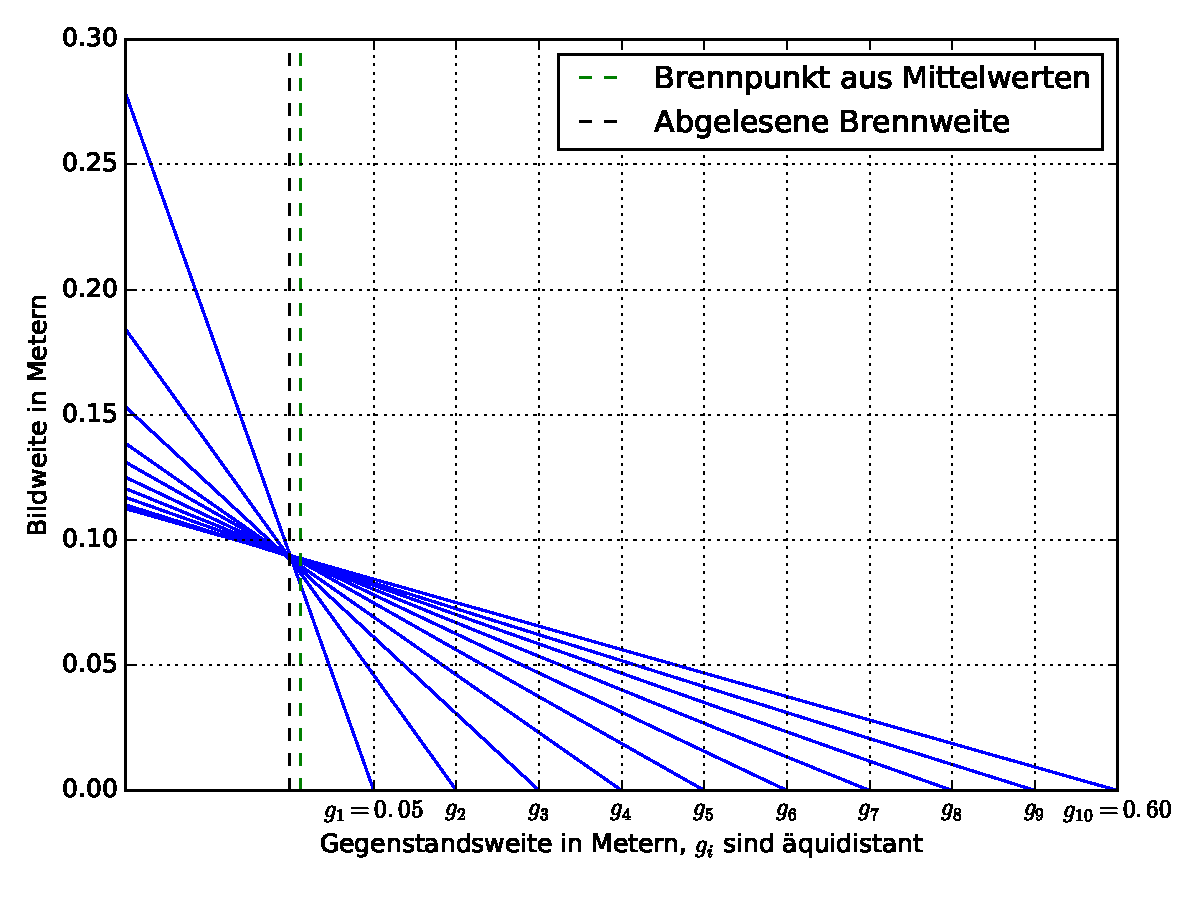
\includegraphics[width=\textwidth]{Messung1_brennnweite_bekannt.pdf}
  \caption{Wertepaare $(g_i|b_i)$ aufgetragen. Zudem ist der Mittelwert der gemessenen Brennweite, sowie der abgelesene Schnittpunkt der Geraden eingetragen.}
  \label{fig:brennweite_bekannt}
\end{figure}

Der Schnittpunkt der Geraden im Diagramm \ref{fig:brennweite_bekannt}
ist mit Hilfe des Mauscoursers abgelesen worden. Der Ablesefehler wird mit
$\SI{0,3}{\centi\meter}$ angegeben.
Der Schnittpunkt hat einen Wert von $S_1 = (\num{99(3)e-1}|\num{94(3)e-1})$.
Die Angaben sind in Centimetern.

Desweiteren wurde die Brennweite einer unbekannten Linse bestimmt.
Es wurde gleich verfahren, wie bei der Messung der bekannten Linse.
Die Messdaten sind in Tabelle \ref{tab:unbekannte_brennweite} dargestellt.

\begin{description}
  \centering
  \item[$<f_2>\ua{gemessen}=$]\SI{9028(3)e-2}{\centi\meter}
\end{description}

Das Diagramm \ref{fig:unbekannte_brennweite} zeigt die Verbindungsgeraden,
der Wertepaare der gemessenen $(g_i|b_i)$.

\begin{figure}
  \centering
  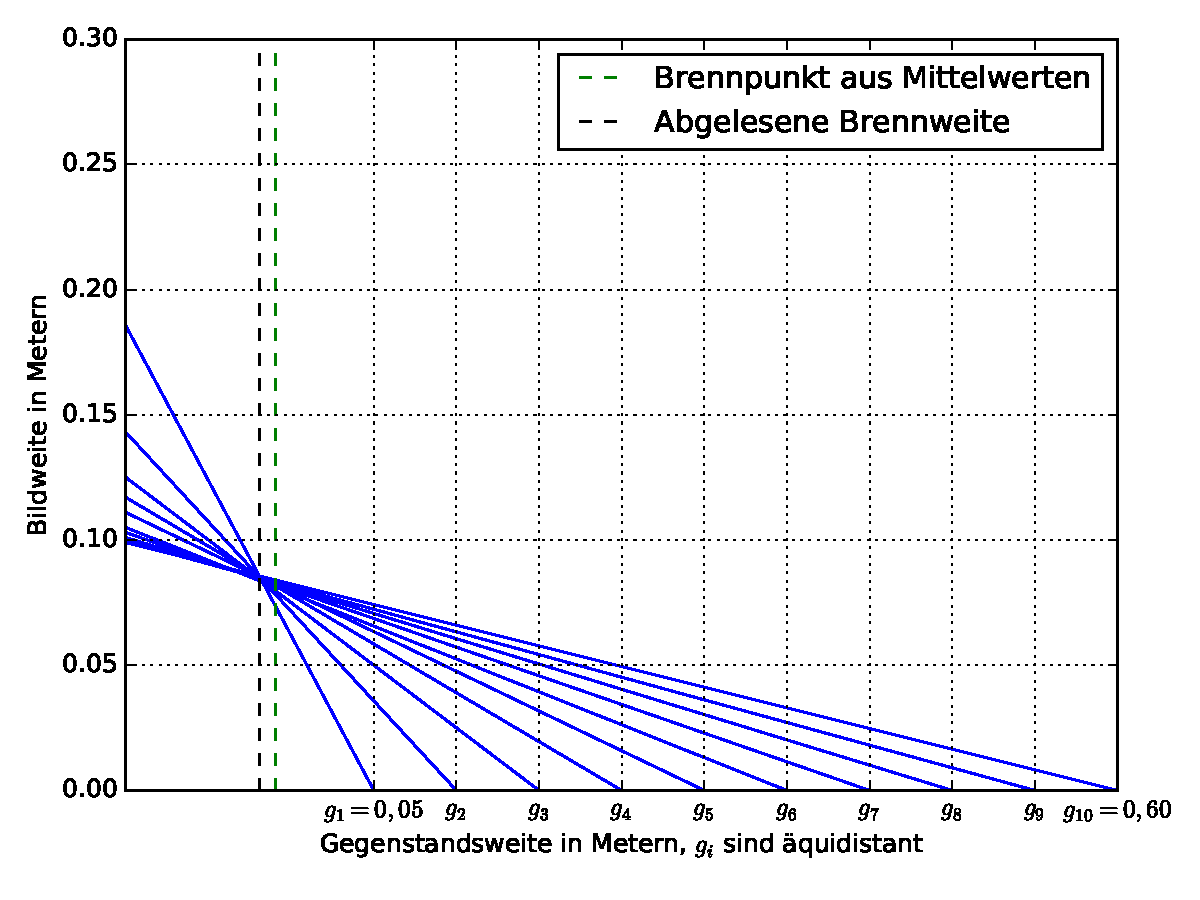
\includegraphics[width=\textwidth]{Messung2_unbekannte_brennweite.pdf}
  \caption{Wertepaare $(g_i|b_i)$ aufgetragen. Zudem ist der Mittelwert der gemessenen Brennweite, sowie der abgelesene Schnittpunkt der Geraden eingetragen.}
  \label{fig:unbekannte_brennweite}
\end{figure}

Der abgelesene Schnittpunkt ist gegeben mit $S_2 =
(\num{81(3)e-1}|\num{84(3)e-1})$. Die Angaben sind in Centimetern.

\begin{table}
\centering
\caption{Messdaten der Linse mit unbekannter Brennweite.}
\label{tab:unbekannte_brennweite}
\begin{tabular}{S S}
\toprule
{$g$ in $\si{\centi\meter}$} & {$b$ in $\si{\centi\meter}$} \\
\midrule
15 & 18.55 \\
20 & 14.30 \\
25 & 12.50 \\
30 & 11.70 \\
35 & 11.10 \\
40 & 10.50 \\
45 & 10.30 \\
50 & 10.10 \\
55 & 9.95  \\
60 & 9.90  \\
\bottomrule
\end{tabular}
\end{table}


Die Messgrößen in Tabelle \ref{tab:unbekannte_brennweite} haben alle den Ablesefehler
$\SI{0,05}{\centi\meter}$.

\subsection{Bestimmung der Brennweite nach Bessel}

Die Messdaten der Messung sind in Tabelle \ref{tab:bessel} dargestellt.
Damit der Datensatz größer ist, werden die Messdaten
von $b_1, g_1$ und $b_2, g_2$ verwendet. Theoretisch sind $b_1 = g_2$
und $b_2 = g_1$ identisch.

Die Mittelwerte der Messdaten wurden in die Formel \eqref{eqn:} eigetragen.
Daraus ergibt sich die folgende Brennweite.

\begin{equation}
  \centering
  \label{eqn:bessel_ergebnis}
  f\ua{Bessel}= \SI{9,67}{\centi\meter}
\end{equation}

Der Fehler von \eqref{eqn:bessel_ergebnis} ist, bezüglich der Messgenauigkeit,
vernachlässigbar klein und wird daher weggelassen.

\begin{table}
\centering
\caption{Messdaten der Methode nach Bessel}
\label{tab:bessel}
\begin{tabular}{S S S S S S }
\toprule
{$e$ in $\si{\centi\meter}$} & {Fehler $e$} & {$g_1$ in $\si{\centi\meter}$} & {Fehler $g_1$} & {$g_2$ in $\si{\centi\meter}$} & {Fehler $g_2$}  \\
\midrule
 40  & 5.00  & 16.6  & 5.00  & 23.70  & 5.00\\
45  & 5.00  & 14.2  & 5.00  & 31.05  & 5.00\\
50  & 5.00  & 13.2  & 5.00  & 37.00  & 5.00\\
52  & 5.00  & 12.9  & 5.00  & 40.00  & 5.00\\
55  & 5.00  & 12.6  & 5.00  & 42.60  & 5.00\\
58  & 5.00  & 12.4  & 5.00  & 45.35  & 5.00\\
60  & 5.00  & 12.2  & 5.00  & 48.00  & 5.00\\
62  & 5.00  & 12.2  & 5.00  & 50.75  & 5.00\\
65  & 5.00  & 12.0  & 5.00  & 53.35  & 5.00\\
70  & 5.00  & 11.8  & 5.00  & 58.45  & 5.00\\
\bottomrule
\end{tabular}
\end{table}


Die Messgrößen in Tabelle \ref{tab:bessel} haben alle den Ablesefehler
$\SI{0,05}{\centi\meter}$.

Darüberhinaus wurde die chromatische Abberration untersucht.
Die Messdaten sind in Tabelle \ref{tab:chromatische_abberration} dargestellt.

\begin{align}
  \label{eqn:rot}
  f\ua{rot} &= \SI{967(1)e-2}{\centi\meter}\\
  \label{eqn:blau}
  f\ua{blau} &= \SI{966e-2}{\centi\meter}
\end{align}

Der Fehler bei \eqref{eqn:blau} ist, bezüglich der Messungenauigkeit,
zu vernachlässigen.

\begin{table}
\centering
\caption{Messdaten zur chromatischen Abberration}
\label{tab:chromatische_abberration}
\begin{tabular}{S S S S S S S S S S }
\toprule
{$e$ in $\si{\centi\meter}$} & {Fehler $e$} & {$g_{1,\symup{rot}}$ in $\si{\centi\meter}$} & {Fehler $g_{1,\symup{rot}}$} & {$g_{2,\symup{rot}}$ in $\si{\centi\meter}$} & {Fehler $g_{2,\symup{rot}}$} & {$g_{1,\symup{blau}}$ in $\si{\centi\meter}$} & {Fehler $g_{1,\symup{blau}}$} & {$g_{2,\symup{blau}}$ in $\si{\centi\meter}$} & {Fehler $g_{2,\symup{blau}}$} \\ 
\midrule
 45  & 5.00  & 14.35  & 5.00  & 31.0  & 5.00  & 14.10  & 0.00  & 31.2  & 0.00\\
50  & 5.00  & 13.20  & 5.00  & 37.0  & 5.00  & 13.25  & 0.00  & 37.1  & 0.00\\
55  & 5.00  & 12.60  & 5.00  & 42.5  & 5.00  & 12.70  & 0.00  & 42.7  & 0.00\\
60  & 5.00  & 12.35  & 5.00  & 48.1  & 5.00  & 12.40  & 0.00  & 48.2  & 0.00\\
65  & 5.00  & 12.00  & 5.00  & 53.5  & 5.00  & 12.10  & 0.00  & 53.3  & 0.00\\
\bottomrule
\end{tabular}
\end{table}


Die Fehler von $e$, $g\ua{1,rot}$, $g\ua{2,rot}$, $g\ua{1,blau}$ und $g\ua{2,blau}$
betragen jeweils $\SI{0,05}{\centi\meter}$.

\subsection{Bestimmung der Brennweite von Linsensystemen nach Abbe}

Die Messdaten der Messung sind in Tabelle \ref{tab:abbe} dargestellt.
Mit Formel \eqref{eqn:} ergeben sich daraus die folgenden Werte.

\begin{align}
  \label{eqn:brennweite_abbe_g}
  f\ua{g} &= \SI{1693(32)e-2}{\centi\meter} \\
  \label{eqn:hauptebene_h}
  f\ua{h} &= \SI{-938(95)e-2}{\centi\meter}\\
  \label{eqn:brennweite_abbe_b}
  f\ua{b} &= \SI{1442(17)e-2}{\centi\meter} \\
  \label{eqn:hauptebene_abbe_h_strich}
  f\ua{h´} &= \SI{1305(31)e-2}{\centi\meter}
\end{align}

\begin{figure}
  \centering
  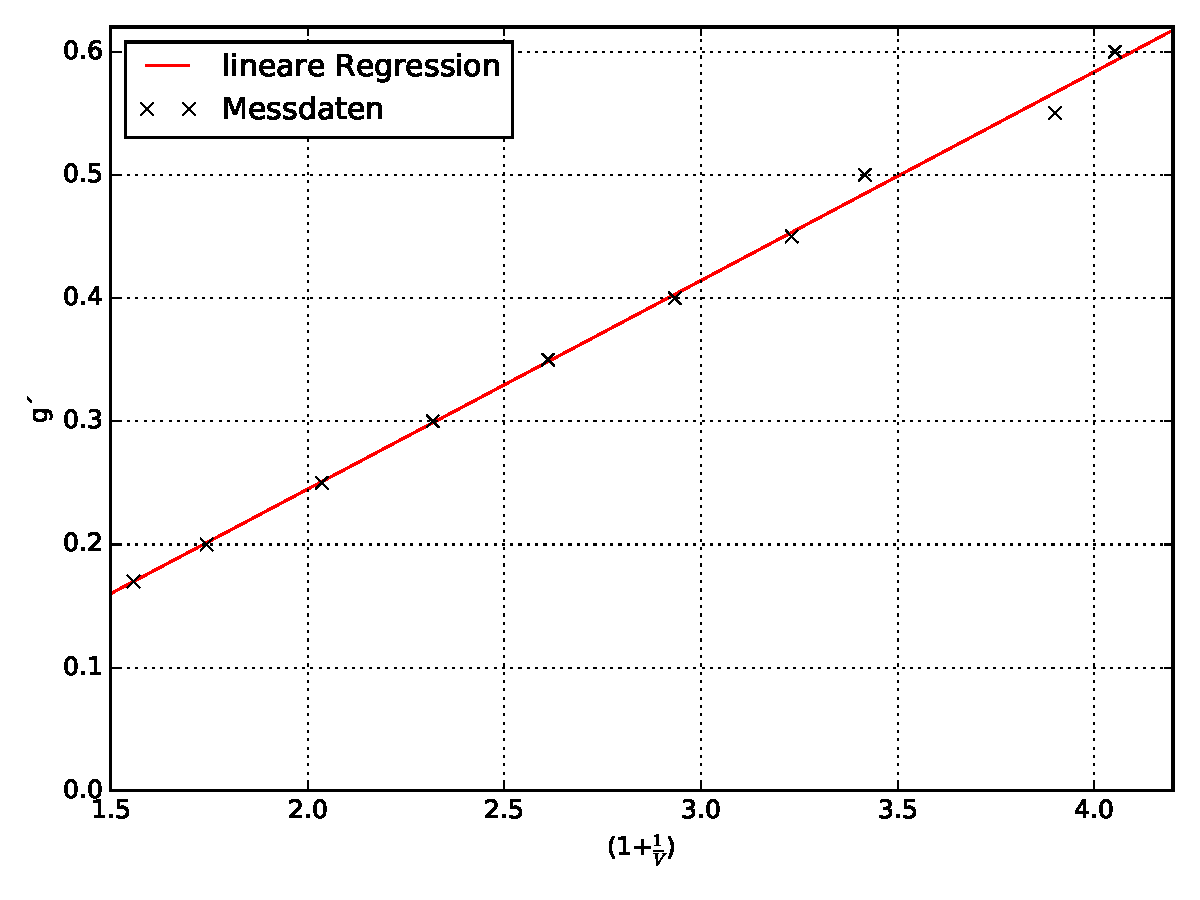
\includegraphics[width=\textwidth]{Messung_abbe_g.pdf}
  \caption{Wertepaare $(1 + \frac{1}{V_i}|g_i)$ mit linearer Regression.}
  \label{fig:abbe_g}
\end{figure}

\begin{figure}
  \centering
  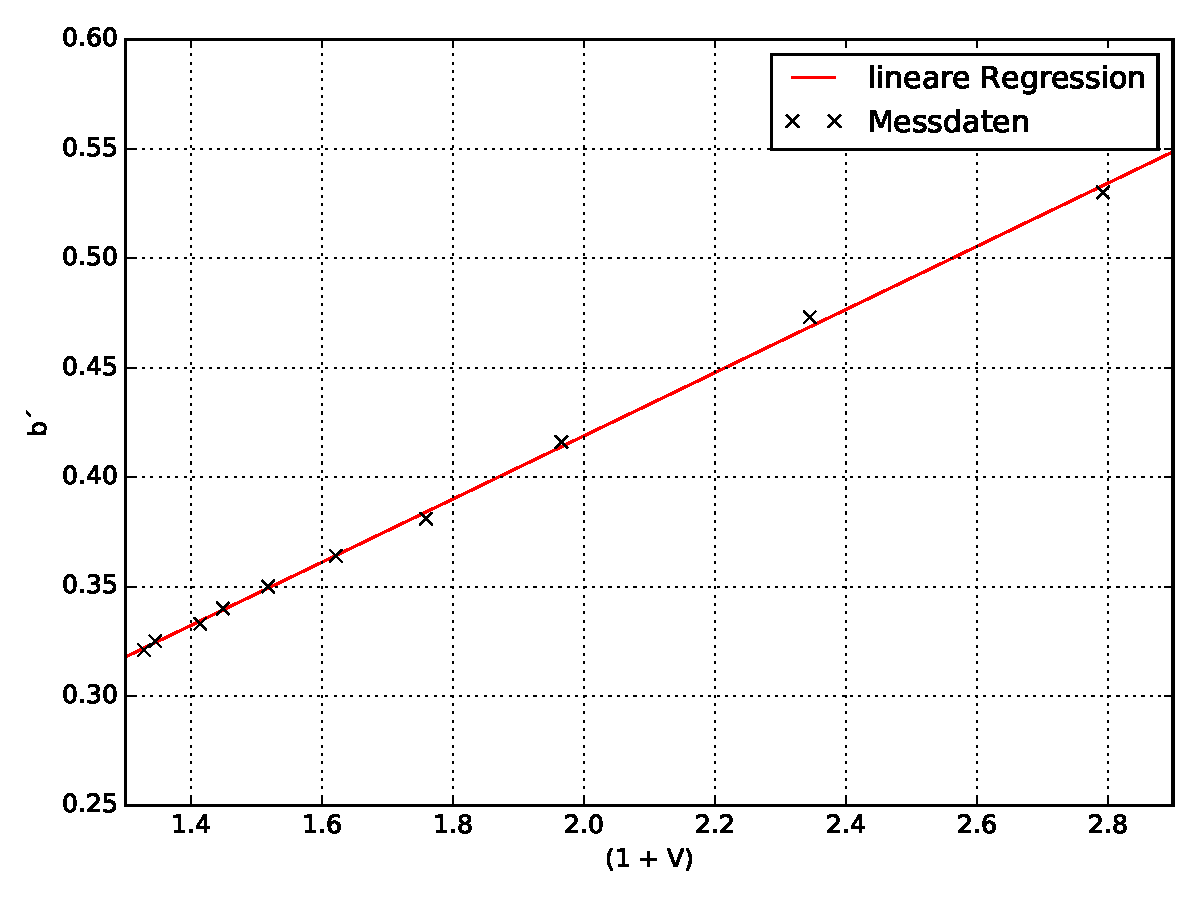
\includegraphics[width=\textwidth]{Messung_abbe_b.pdf}
  \caption{Wertepaare $(1 + V_i|b_i)$ mit linearer Regression.}
  \label{fig:abbe_b}
\end{figure}

\begin{table}
\centering
\caption{Messdaten der Methode nach Abbe}
\label{tab:abbe}
\begin{tabular}{S S S S S S }
\toprule
{Bildgröße $B$ in $\si{\centi\meter}$} & {Fehler $B$} & {$b + g$ in $\si{\centi\meter}$} & {Fehler $g + b$} & {$g$ in $\si{\centi\meter}$} & {Fehler $g$} \\
\midrule
 5.2  & 5.00  & 70.0  & 5.00  & 17  & 5.00\\
3.9  & 5.00  & 67.3  & 5.00  & 20  & 5.00\\
2.8  & 5.00  & 66.6  & 5.00  & 25  & 5.00\\
2.2  & 5.00  & 68.1  & 5.00  & 30  & 5.00\\
1.8  & 5.00  & 71.4  & 5.00  & 35  & 5.00\\
1.5  & 5.00  & 75.0  & 5.00  & 40  & 5.00\\
1.3  & 5.00  & 79.0  & 5.00  & 45  & 5.00\\
1.2  & 5.00  & 83.3  & 5.00  & 50  & 5.00\\
1.0  & 5.00  & 87.5  & 5.00  & 55  & 5.00\\
0.9  & 5.00  & 92.1  & 5.00  & 60  & 5.00\\
\bottomrule
\end{tabular}
\end{table}


Die Messgrößen in der Tabelle \ref{tab:abbe} haben alle den Ablesefehler
von $\SI{0,05}{\centi\meter}$

\section{Diskussion}

Anfangs ist zu erwähnen, dass die Grad der Bildschärfe per Hand, und somit
nur subjektiv bestimmt werden konnte. Damit ist anzunehmen, dass die Messergebnisse
auf Grund des Messverfahrens fehlerbehaftet sind.
Im Folgendem werden die Messergebnisse hinsichtlich ihrer Aussagekraft diskutiert.

Die Messgenauigkeit der Brennweitenmessung ist in Diagramm
\ref{fig:brennweite_bekannt} einzusehen. Bei einer hohen Messgenauigkeit haben
die eingetragenen Geraden einen gemeinsamen Schnittpunkt. Dies ist, unter
Berücksichtigung der Messunsicherheit, erreicht worden. Die Messergebnisse
werden sind als präzise einzustufen. Die Messung weicht lediglich um
$\approx\SI{0,5}{\centi\meter}$ von der angegebenen Brennweite ab. Dies ebenfalls
auf eine hohe Präzision der Messung hin.

Als Linse mit unbekannter Brennweite, wurde eine befüllbare Linse genommen. Über eine
Spritze mit Wasser konnte die Befüllung der Linse reguliert werden.
Damit in der Linse ein konstanter Druck gewährleistet wurde, musste die Spritze an
einer definierten Person fixiert werden.
Die Fixierung wurde per Hand bewerkstelligt. Die Messung war länger, womit
ein dauerhaft konstanter Druck unwahrscheinlich scheint. Dadurch können
die Messung beeinflusst worden sein. Der in Diagramm
\ref{fig:unbekannte_brennweite} entstandene Schnittpunkt, weißt hingegen auf eine
hohe Messgenauigkeit hin.

Die Messung der Linse mit unbekannter Brennweite ergab eine Brennweite von ca. $\SI{9,03}{\centi\meter}$.
Die Messgenauigkeit ist in Abbildung \ref{fig:unbekannte_brennweite} einzusehen.
Anhand des Schnittpunktes der Verbindungsgeraden ist die Messgenauigkeit im Rahmen
der Messung als präzise zu bewerten.

Die chromatische Abberration ergab, dass die Brennweite bei blauer Lichtquelle
minimal kleiner ist, als bei roter Lichtquelle. Dies entspricht der Erwartung.
